\documentclass{report}
\usepackage{amsmath}
\usepackage{relsize}
\usepackage{graphicx}
\graphicspath{ {images/} }
\usepackage{comment}
\usepackage{notes}
\usepackage{color}
\usepackage{hyperref}
\begin{document}
\linespread{1.6}
%\renewcommand{\baselinestretch}{1.5}
\begin{titlepage}

\newcommand{\HRule}{\rule{\linewidth}{0.5mm}} % Defines a new command for the horizontal lines, change thickness here

\center % Center everything on the page
 
%----------------------------------------------------------------------------------------
%	HEADING SECTIONS
%----------------------------------------------------------------------------------------


\includegraphics{logo_blau}\\[1cm]
%\textsc{\LARGE Technical University of Dresden}\\[1.5cm] % Name of your university/college
\textsc{\Large Master thesis}\\[0.5cm] % Major heading such as course name
\textsc{\large Database Group}\\[0.5cm] % Minor heading such as course title

%----------------------------------------------------------------------------------------
%	TITLE SECTION
%----------------------------------------------------------------------------------------

\HRule \\[0.4cm]
{ \huge \bfseries Bit flip detection in Prefix trees}\\[0.4cm] % Title of your document
\HRule \\[1.5cm]
 
%----------------------------------------------------------------------------------------
%	AUTHOR SECTION
%----------------------------------------------------------------------------------------

\begin{minipage}{0.4\textwidth}
\begin{flushleft} \large
\emph{Author:}\\
Mina Ahmadi % Your name
\end{flushleft}
\end{minipage}
~
\begin{minipage}{0.47\textwidth}
\begin{flushright} \large
\emph{Supervisors:} \\
Prof. Dr.-Ing Wolfgang Lehner, Dr.-Ing. Dirk Habich, Dipl.-Inf. Till Kolditz  % Supervisor's Name
\end{flushright}
\end{minipage}\\[4cm]

% If you don't want a supervisor, uncomment the two lines below and remove the section above
%\Large \emph{Author:}\\
%John \textsc{Smith}\\[3cm] % Your name

%----------------------------------------------------------------------------------------
%	LOGO SECTION
%----------------------------------------------------------------------------------------

%
\includegraphics{logo_blau}\\[1cm] % Include a department/university logo - this will require the graphicx package

%----------------------------------------------------------------------------------------
%	DATE SECTION
%----------------------------------------------------------------------------------------

{\large{November 2015}}\\[3cm] % Date, change the \today to a set date if you want to be precise
 
%----------------------------------------------------------------------------------------

\vfill % Fill the rest of the page with whitespace

\end{titlepage}

%\specialcomment{notes}{\begingroup\sffamily\color{red}}{\endgroup}

\tableofcontents

\chapter{Introduction}

\section{Motivation}

Bit flip is an inevitable concept in the memories. Bit flips can happen in the instructions or in the data in the memory. This can cause changing the control flow of the program or can change data which is going to be read or written from and into memory. If bit flips happen in the index-structures of databases, then we will retrieve wrong values or even access a part of memory which has not been allocated for our data and get segmentation fault error. Detecting bit flips in memory is a vital task to do. Different index structures are introduced for keeping indexes of tables in databases. We would like to find bit flips which occurs in prefix trees.  

\section{Objectives}

Finding bit flips in Prefix trees-which is one type of index structure that is used for keeping indexes- is the main objective of this thesis. We would like to achieve a good performance at the end. For this purpose, we will use a few techniques for bit flip detection and will show the result of each technique and will do an evaluation to compare these techniques.

\section{Structure}

In the second chapter, some background knowledge about some terms is given and also the related works are mentioned and are explained in details.

In the third chapter the concept of this thesis is given. The strategies which are used to reach the objectives of the thesis are explained in details and a brief conclusion of them is given. 

In the implementation chapter, all the implementation details of the methods which are used is given. 

Finally, in the last chapter, conclusion and some evaluations are given to show the result of the used methods. 

\chapter{Background and Related works}

In this section, a brief explanation of some terms are given and also a number of works which are already done and are related to this thesis have been analysed.

\section{Background}

\subsection{What is bit flip?}

Any change in the bits which are stored in the memory is called bit flip. If binary 1 changes to 0 or 0 changes to 1, then bit flip has happened.

\subsection{Types of error}

Bit flips that happen in the memory are divided into two groups. They can be soft or hard errors.

\begin{enumerate}

\item \textbf{Hard errors}: If a failure happens in a memory chip, then we might have hard errors. These type of errors will be fixed in the memory and the only solution is to replace the chip. One of the causes of having hard errors is having system functions over the limit of the memory's speed. \cite{harderror}

\item \textbf{Soft errors}: These types of errors do not cause any failure in the hardware. These errors will change the data in the memory. By starting over the PC, the error will go away.\cite{softerror} There are a couple of situations which lead to soft error.
\begin{itemize}
\item It happens when radio actives in the chip's material go bad. Some alpha particles will be released which can change the data in a cell.\cite{softerror}
\item It happens when data is being processed. Data can be hit by noise and noise can be interpreted as data bits. \cite{softerror}
\end{itemize}

\end{enumerate}


\subsection{Soft errors' detection mechanisms}

There are some hardware and software mechanisms for detecting soft errors which are listed below.
\begin{description}

\item[Hardware-based techniques] Some hardware-based multi threading techniques \cite{reinhardt,mukherjee,vijaykumar} exist which will execute the application multiple times and the outputs are compared to identify errors. This can cause hardware's design complexity and high cost and performance overhead. \cite{soft} 

\item [Immunity-aware programming] Immunity-aware programming is used when a firmware is going to be programmed for a system. This will improve the tolerance towards soft errors in modules of the program or in program counter. This technique can be used in the software which is written in the source or in the victim device. \cite{immune}

\item [RAM parity memory]  Storing one bit of data as parity which can be even or odd. Parity bit is usually calculated for one byte of data. While reading data from memory, based on the parity bit which is stored, bit flips can be detected. As an example if the data byte is as follows:

11001000

Then:

Parity odd:  0
Parity even: 1

Parity bit used to be stored in an extra memory chip, but now we have DIMM(Dual in-line memory module) and SIMM(Single in-line memory module) which can be found in parity and non-parity modules.\cite{ramparity}

\item [ECC memory] By using Error-correcting code or parity bit as redundant data, single bit errors can be detected. The example of ECC can be single-error correction and double-error detection (SECDED) Hamming code allows correction of one bit and detection of two bits. ECC is used in systems were corruption is not accepted. When systems are not critical, motherboards and processors will not support ECC in order to reduce the expenses. Using ECC memory will be more expensive because producing ECC memory modules and having motherboards and processors which are compatible with ECC memory is expensive. Memory performance will be decreased a bit because ECC memory controllers need to do some calculations for error checking. \cite{eccmemory}

\end{description}

After giving an overview about bit flips and mechanisms for detecting them, we put our focus on the bit flips that happen in index structures of the databases and how to detect them.
 
In the next section of this chapter, based on the related works, we give an overview of the index structures and some detection mechanisms which are given for them. 

\section{Related works}

\subsection{A study of Index Structures for Main Memory Database Management Systems  \cite{leca} }

In this paper, different types of in-memory index structures have been explained and compared with each other and a new index structure called as T tree has been introduced.
The main goal for an index structure in disk is to minimize the disk accesses, but the goal for an index structure in memory is to emphasize on the use of CPU cycles and less usage of memory. Since all the relations are in the memory, it is not needed to keep the values according to each index. Instead, the pointer to the values can be kept. For example if we are using a tree structure to keep the indexes, if we were supposed to keep the values according to each index, then we might have nodes with different sizes since the length of the values were different.
\subsubsection{Array}

The size of the structure is fixed. The main disadvantage is that for each delete or insert operation, $\mathcal{O}(\log{}N)$ is the complexity.

\subsubsection{AVL trees}

The structure in a AVL tree is like a binary search tree and if an insertion or deletion cause an imbalance in the tree, a rotation will be done in the tree to keep the tree balanced again. The disadvantage is the bad memory utilization, since each nodes will hold one item and two pointers.
 
\subsubsection{B trees}

Unlike AVL trees, the depth of the tree is less and less number of nodes need to be accessed while searching for an index. Insertion and deletion is also fast.

\subsubsection{Chained Bucket Hashing}

This structure is static and size of it is fixed. The operations are fast but if the size of the structure is fixed to a small size, then it can cause problems in the performance. Assuming a large size for the structure can cause unnecessary usage of memory.

\subsubsection{Extendible Hashing}

Unlike \textit{Chained bucket hashing}, this structure is dynamic. Whenever a new data is going to be added, if the corresponding node has space, it will be added there. Otherwise, the node will split. If split is not possible on a node, then the directory size has to increase. For example if directory has 00,01,10,11 as the prefixes and we have to increase the directory size, then we will have 000,001,010,011,100,101,110,111 as the prefixes. The problem with this approach is that insertion of a node can cause enlargement of the directory.  

\subsubsection{Linear Hashing}

This is also a dynamic structure. The directories are not separate from the keys, but the keys are kept inside the directories. After adding each node,  splitting of the node should be decided. If the result of the following equation is greater than $75\%$, then the node should be split:

\begin{equation}
\frac{Number of keys}{Number of buckets * Size of the bucket} \\
\end{equation}   
In Linear hashing, splitting a node is done in a more organized way than \textit{Extendible hashing}.

\subsubsection{T tree}

The structure of T tree is a combination of AVL tree and B tree. It is a binary tree and needs balancing like AVL tree and each node can have multiple keys like B tree.

The search in T tree is like the search in a binary tree, but we have to compare the value with the greatest value and the lowest value in the node.

 In insertion, the suitable node for inserting the new value should be found, if there is space in that node, we insert the new value and insertion is done. If there is no place for adding the new value, the minimum value in this node will be removed, and then the insertion of new value is done. Then minimum value will be added to the tree. Also in an iteration from the node which has the new value to the leaf, the new value should replace the greatest lower bound value for this node. In case we could not find any node to insert the new value in, then the insertion is done in the last node on that path.(if the value fits into that node, otherwise, a new leaf is added and the new value will be inserted into this node. After adding a new leaf, the tree should be checked for its balance)
 
Based on the tests that are done in this paper, "AVL trees and arrays do not have sufficiently good performance/storage characteristics for consideration as main memory indices" \cite{leca}. T tree seems the best solution for indexing so far. 

\subsection{Prefix B-trees \cite{R.Bayer} }


\subsection{KISS-Tree: Small Latch-Free In-Memory Indexing on Modern Architectures \cite{Kissinger} }

In this paper, KISS tree is presented which is a latch free, in-memory index structure for minimizing number of memory accesses. Structure of KISS tree is like prefix tree with adding compression scheme and virtual memory management.

KISS tree structure has formed of three levels. In prefix tree, key is divided into groups of bits which has equal size, but in KISS tree this is not the case. In KISS tree, we have assumed that keys are 32 bits and size of each group of bits is different and it depends on the level.

\begin{itemize}
 
 \item \textbf{Level 1-Virtual level} In this level, we get the address of the node in the next level through the 16 most significant bit in the key. Nodes in the next level should be stored sequentially. Since there are no nodes in this level, this level is called virtual level.
 \item \textbf{Level 2-On-demand level} The next 10 bits of the key defines the bucket in the node in this level. Based on what was said in the first level, we would like to have the nodes sequentially. On demand allocation is done in this level, so we have allocated large amount of memory in virtual address space, but when we write something into the node, then a part of physical memory will be allocated for the node. It makes sense to have the node sizes in this level as 4KB, because pages are allocated in memory in 4KB sizes. Each node in this level has ${2}^{10}$ buckets. So the address that should be stored in the bucket should have 4 Bytes. For this reason, compact pointer was introduced to reduce the size of pointer from 64 bits to 32 bits.
  
 \item \textbf{Level 3-compressed node} In this level, 6 bits are left from the key, so the number of buckets inside the nodes is 64 buckets. The compression is done on the nodes in this level. 64 bits is located at the start of each node which defines which of the buckets are used. We do not have to allocate 64 buckets at once. 
 
\end{itemize}    

\subsubsection{Operations}

\begin{itemize}

\item \textbf{Update} As an example, if we would like to insert key 42 into the tree, then with the first 16 bits of the key, we identify the node in the next level. We use the next 10 bits of the key to identify the bucket inside the node. All the pointers in the node are zero, so the node is not physically allocated in the memory. Then we have to ask for a node from memory to insert the bit map and one value. Then we have to set the bit in bitmap which is defined by the third part of the key which in this case is 42. Then we write the value after bitmap in the node. Then we have to set the pointer in the second level with the compact pointer. 

\item \textbf{Read} Then for reading key 42 from the tree, we will identify the node in the next level through the first 16 bit of the key and we identify the bucket using the next 10 bits of the key. Since the bucket is not zero, we get the actual pointer from the compact pointer which is stored in the bucket. In the third level, we find the node and check the 42\textsuperscript{nd} bit of the bitmap in the node, if it is set, we have to get the corresponding value from the node.

\end{itemize}

\subsubsection{Memory management}

At the start, virtual memory is allocated for each of the 64 possible node sizes in the third level. So we can have ${2}^{26}$ blocks of memory, which each of these blocks have a part of memory which is allocated for 64 possible node sizes. An action which is defined in this work is called RCU(read-copy-update). Based on this action, sizes of the nodes in the third level can change, so If another bit in the bitmap of a node is going to bet set as one, then the value should be added to the node, so the size of the node should be changed. In this case, till the new node is created, user can get the value from the old node. When the new node is ready, address of the new node should be set to the corresponding bucket in the second level.    


\subsection{CTrie\cite{ctrie}}

A Ctrie \cite{calfcht,ctenbs}, is a type of \textit{hash array mapped trie} \cite{hamt} which is concurrent and lock-free. The methodology of Ctrie is used in KISS tree's  \cite{Kissinger} implementation. All the operations including insert, remove and search can be done concurrently in Ctrie. Based on the methods in \textit{hash array mapped trie}, hash code of a key is calculated. Each node can have up to 32 fragments. The memory will not be allocated for a node with 32 fragments because some of the fragments can be null pointers. At the start of each node, there is a 32 bits bitmap which defines which of the 32 fragments are set. Then an array with the size of all the ones in the bitmap is allocated. An operation called \textit{compare and swap} (CAS) is done on the node whenever a key is going to be inserted on that node. There are some indirection nodes in between of each node and its sub levels to make sure that the updates are done in the correct way. In the following figure, the initial picture of the tree and picture of the tree after insertion of some keys is given. Whenever there is a key with the same hash code, at least a level should be added into the tree and of course an indirection node is put in between.

\begin{figure}[h]
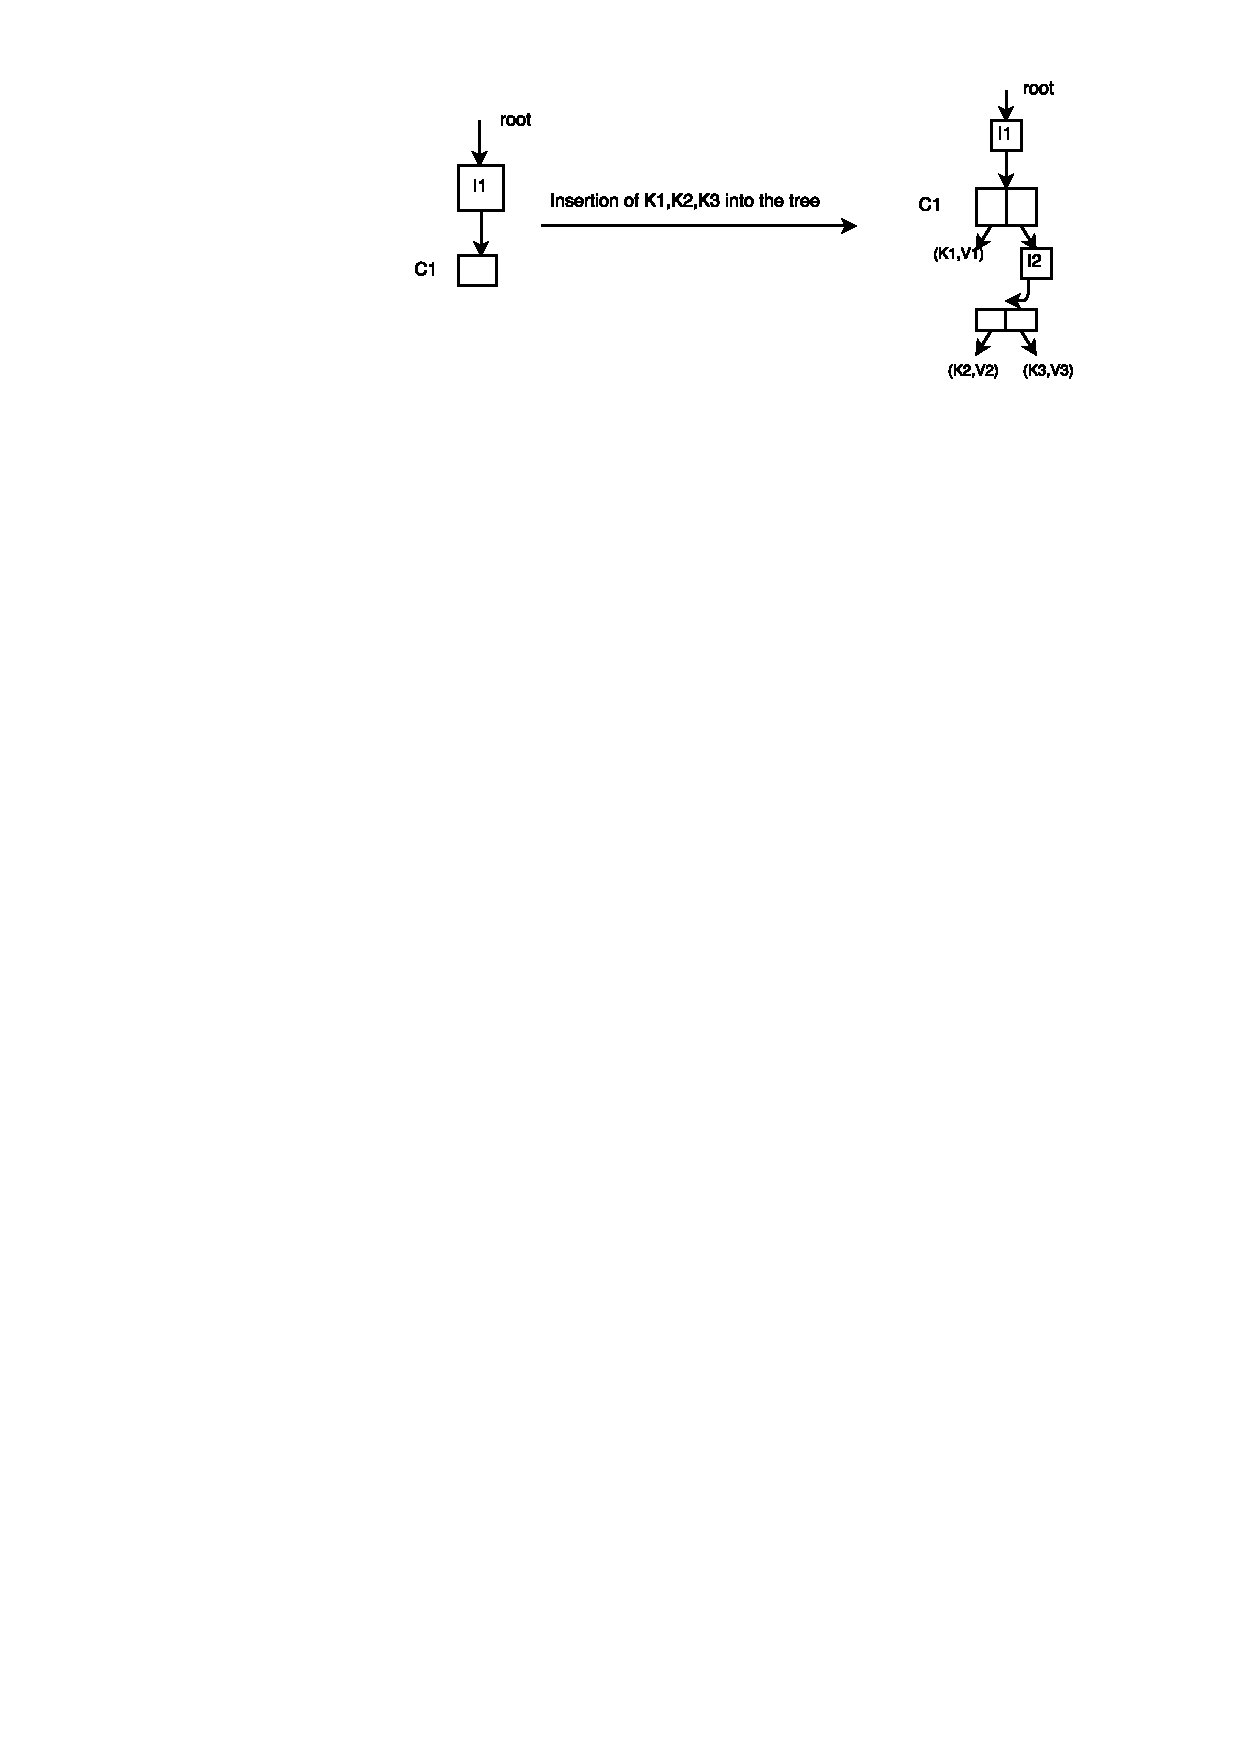
\includegraphics[scale=0.6]{ctrie}
\caption{ Ctrie Insertion}
\centering
\end{figure} 


\subsection{Burst Trie \cite{burst}}

In this paper, Burst trie has been introduced. In comparison with other structures, this structure is not using more memory than hash tables or other tree structures like binary search tree or Splay trees \cite{splay} or ternary search trees. In comparison to Splay trees, Burst trie can store 10 GB of vocabulary in $40\%$ less   time. Burst trie is more efficient than ternary search tree in memory usage and has a better performance.

Search length in tree structures is higher than hash tables. Burst trie aimed on reducing string comparisons to less than two as well as caring about memory consumption.

Structure of Burst trie contains of three main components:
\begin{itemize}

\item[Record] has a unique string which acts as a key. 

\item [Container] has a number of records inside. Data structure which is used inside a container can be a simple data structure like a BST or a list.

\item Access trie
\end{itemize}  


In the following figure, we see a tree after insertion of "came", "car", "cat", "cave", "cy", "cyan", "we", "went", "were", "west".

\begin{figure}[h]
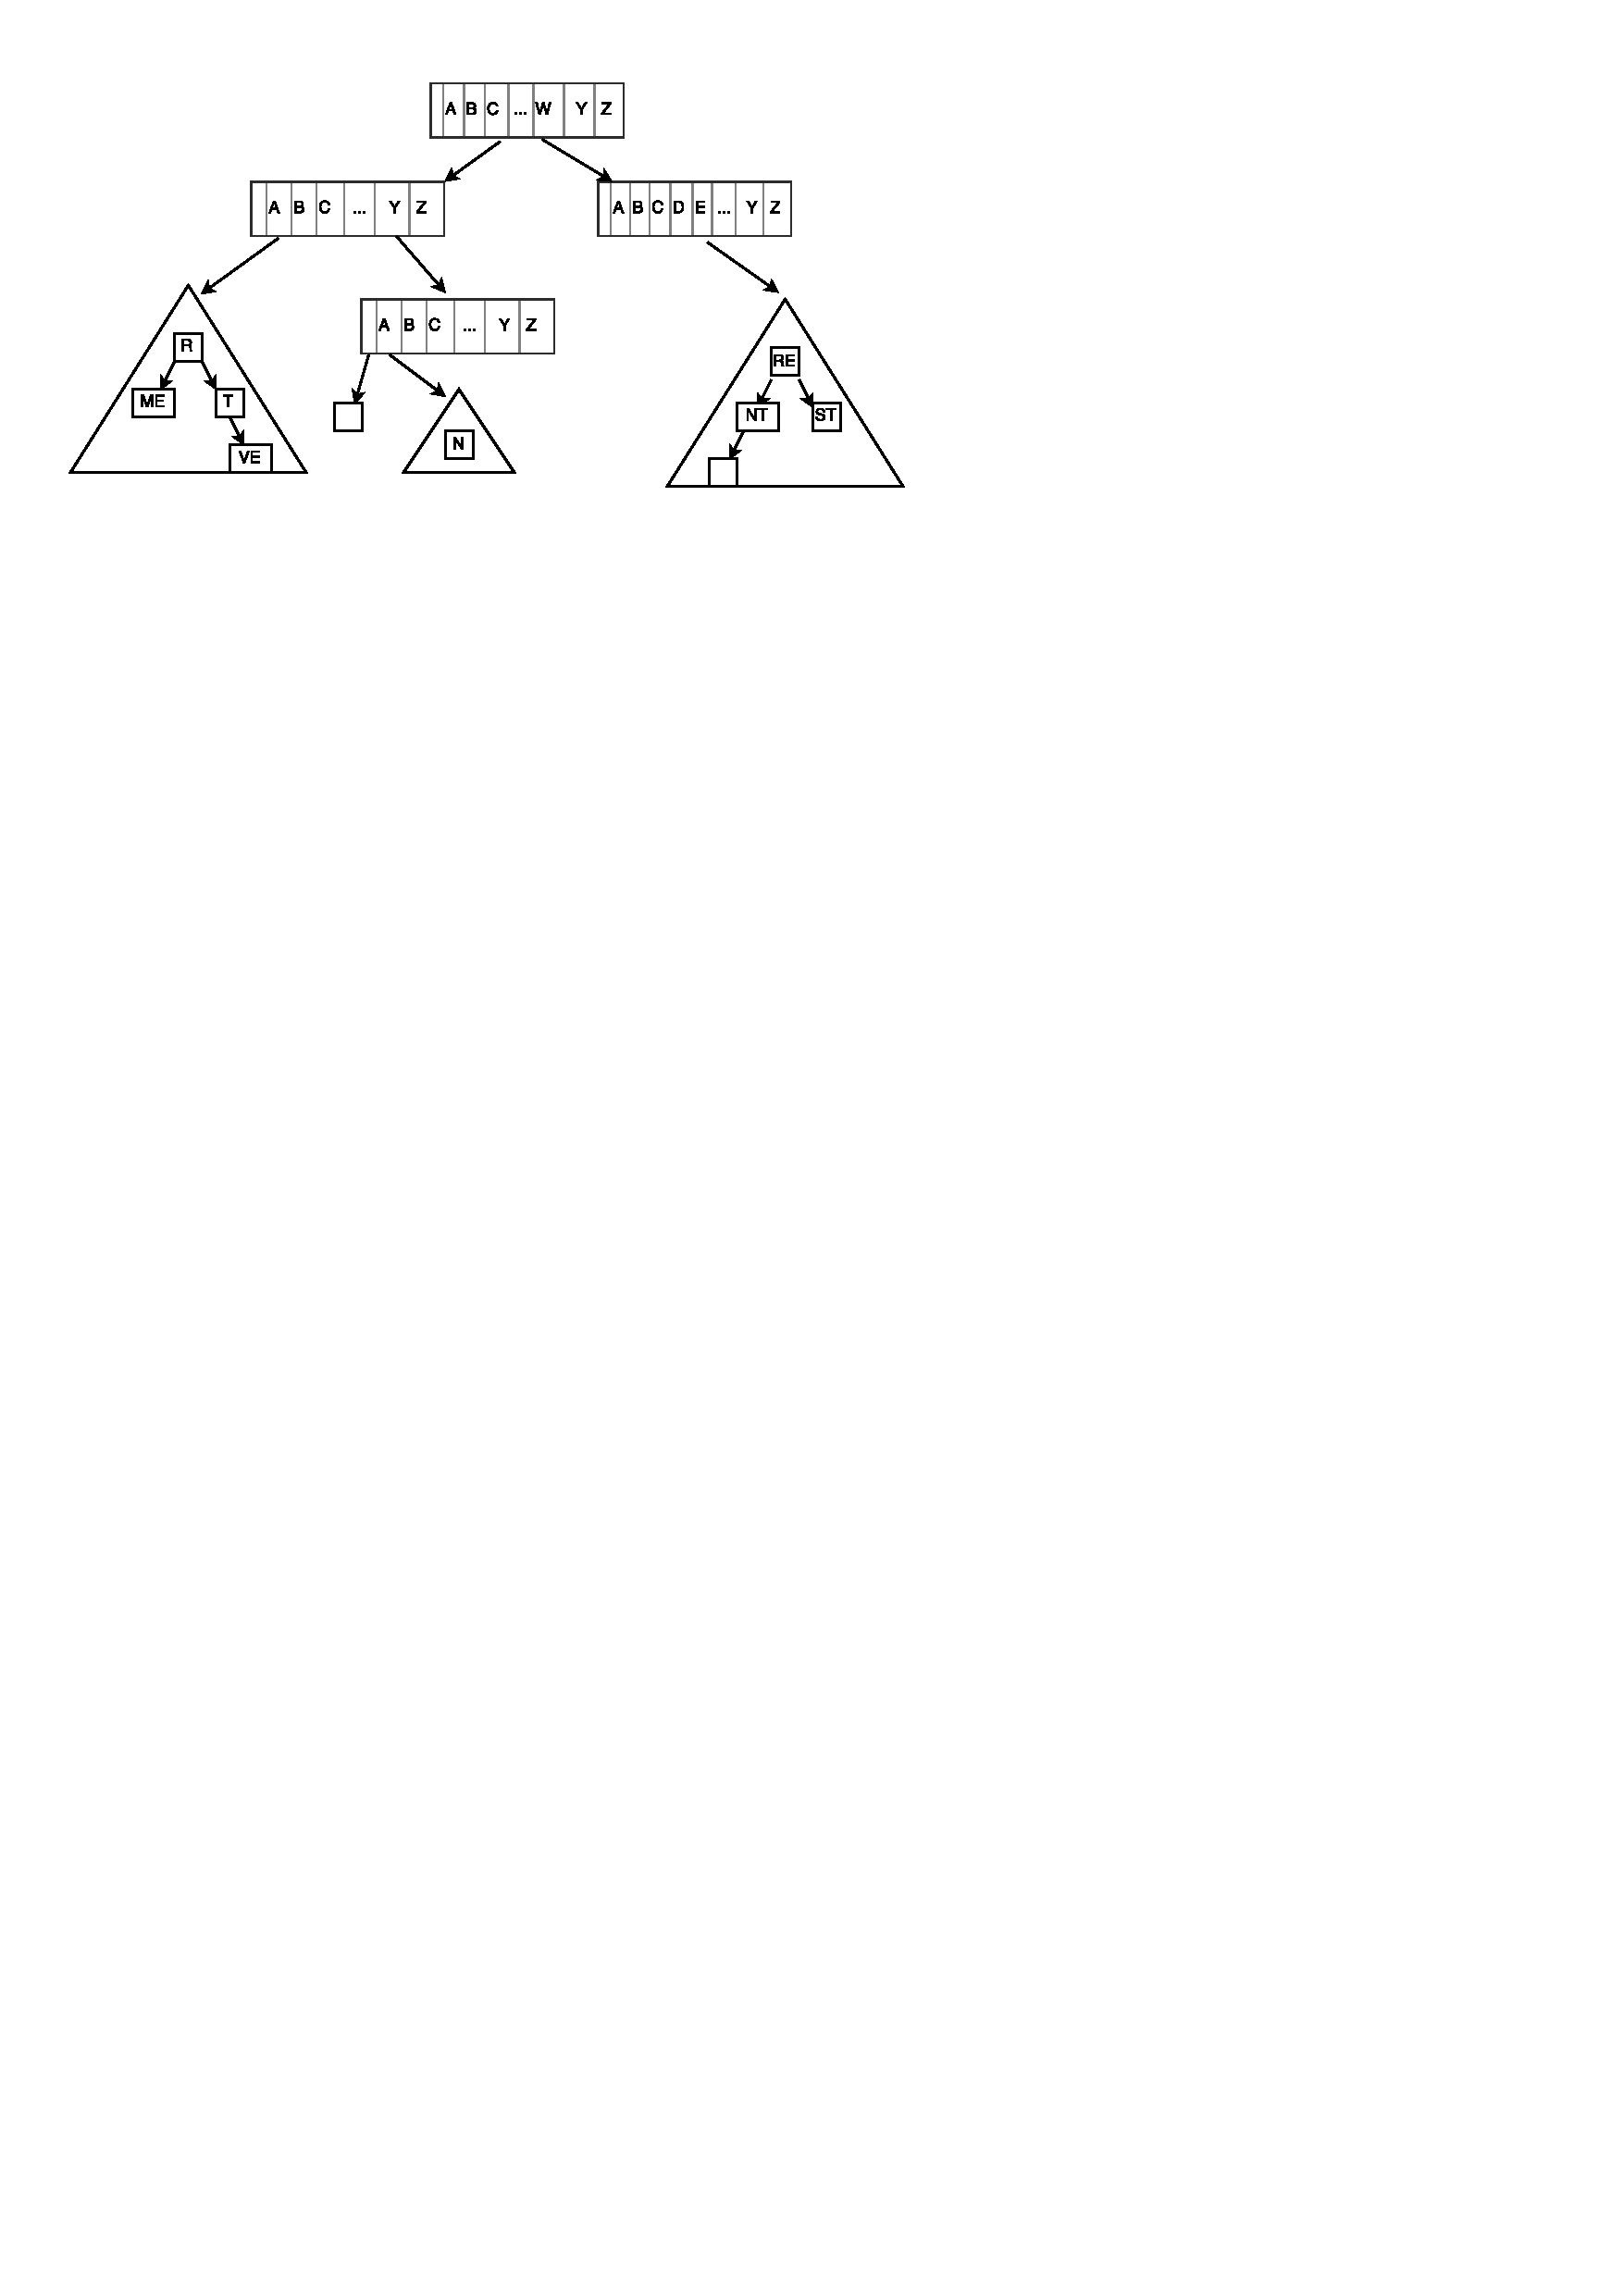
\includegraphics[scale=0.6]{bursttrie}
\caption{ Burst trie after insertion of a number of keys}

\centering
\end{figure}

\subsubsection{Search}

For search in Burst trie, we refer to the root of the trie and find the fragment which has the first character of the word. Then we have to check where does this fragment points to. If it points to a node, we have to continue traversing the same way. At the end if we reach a node which is at level $n+1$(n is the number of characters in a word), we refer to the empty string of that node. If fragment points to a container, then we have to search for the remaining characters of the word by doing a binary search in the container.

\subsubsection{Insertion}

We have to do a correct traverse in order to find the container in which the new key should go. We assume that the found container is at level k. In case $k=n+1$, key should be inserted in the empty string of that node. If k is less than n, then the new key should be inserted into the correct container.

\subsubsection{Bursting}

It happens when a container in level k is replaced by a node and a number of containers which are pointed to from that node. The new containers are located at level $k+1$. All the records which were in the old container should be pointed to from a fragment in the newly created node. 

Based on some experiments which are done on Burst tries, they are memory efficient and faster in comparison with Splay trees, binary trees or tries but still a bit less efficient than hash tables.    


\subsection{Online Bit Flip Detection for In-Memory B-Trees on Unreliable Hardware \cite{kolditz} }

In this paper, B-tree has been chosen for the index structure and various techniques have been introduced for finding bit flips. These techniques can be used in other data structures later.

ECC-DRAM is one of the techniques that exists in order to detect bit flips in the memory, though this technique increases memory consumption The other technique is TMR, to three modules of any structure and then compare the final result with each other and decide based on the majority.This method will obviously increase memory consumption and needs redundant computation. Based on this paper, detection of bit flips is accomplished by using the structure of B-tree and using different levels of redundancy for assuring bit flip detection. The other observation was that the number of bit flips per 8-byte word increased when the modules of the memory were old. In the other experiment, after each run, corrupted bits were corrected. In this experiment, the number of corrupted words decreased in relevance to the first experiment. Based on these experiments, heat is one of the factors in increasing the bit flips in main memory, so some techniques should be used to detect and correct the bit flips. Based on the second experiment, the solution is to correct the bit flips in data after accessing it.


Two experiments have been done on this work. In the first experiment, heat has been employed on the memory and the result was that the number of corrupted words increased with increasing the heat.

The first type of B tree which has been implemented, is the Basic B-tree. Each node in the B-tree contains a number of fields. One of these fields is \textit {fill level} which defines the number of key,value pairs that are currently in the node. In the basic B-tree, \textit {fill level} is checked in order to be in the boundary of 0 and 2K, which K defines the number of key,value pairs in the nodes of the tree. No other checks are done in the basic B-tree.

In TMR B-tree, there exists three replicas of the B-tree and each query will be executed on all the replicas and the results will be compared with each other. When the key is found based on the majority, the value according to the keys should also match. There is a possibility that the results of the two replicas are same but both of the results are actually corrupted.

In order to do an online checking on the B-tree to find the bit flips, EDB-trees(Error Detecting B-trees) are defined, in which the checks are done while traversing the tree and searching for a node. The nodes are kept one after another in the virtual address space, so the start and the end of the area allocated for the tree in virtual memory is predefined. So in case, a pointer is corrupted and points to an address out of this boundary, it can be detected. There are some pointer checks that are done while traversing the tree. The pointers should point to addresses in the specified area. Since the parent's address is kept in the child, this address can be compared with the address of the node that is before the current node in the tress traverse.

The other type of EDB-tree for bit flip detection is EDB-tree PB. In this type of tree, parity bits are used in order to detect bit flips. For all the node fields, Parity bit has been calculated and put in the most significant bit. In each traversal, node member's parity bits are checked. The disadvantage of this implementation is that since one bit of each member is used for parity bit, the number of possible values for each member will decrease.

The other type of EDB-tree for bit flip detection is EDB-tree CS. For each node, 4 checksums have been added. One of them is the XOR result of the parent pointer, fill level and tree level. The second one is the XOR result of all the keys. The third one is the XOR result of all the values and the fourth one is the XOR result of all the pointers. For detecting more corrupted elements, it is better to have checksum for each field in a node, but of course this will cause more memory consumption and higher computational costs. Each of the checksums are validated at different times. Whenever a key or a value is added to the tree, the second and the third checksums should be checked. While traversing in the tree, the fourth checksum is checked.

Based on the tests that have been done in this paper, while injecting 1-5 bit flips per 8-Byte word per millisecond in a period of 300 seconds, the results on different types of implemented B-trees is as follows:

In the basic B-tree implementation, since no data correction is done, the number of errors increase with time. When number of injected bit flips is 5, EDB-tree CS and EDB-tree PB can detect more errors. While injecting 2 or 4 bit flips, error detection of B-tree and EDB-tree PB is almost the same, because even number of bit flips cancel each other. About undetected errors, the result shows that in TMR B-trees, the number of undetected errors is zero.               
  

\subsection{Efficient verification of B-tree integrity \cite{Graefe}}

This paper introduces a number of algorithms which are for B-tree validation and also introduces a new algorithm which takes very little memory.

Verification of B-tree has been divided into some groups in this paper. We should verify the relation between nodes and all of the pointers( which can be the child pointers and the pointers between siblings). In-page verification is another part of the verification Another part of verification is about the relations between the tables.
  
\subsubsection{In-page verification}

What matters in this verification is the verification of information in a single node. It can be done buy using a physical test or checksum. Torn-page is the case, when a node needs to access multiple sectors but the access is not possible. For detecting these torn-pages, detection can be done quite fast.

\subsubsection{Index navigation}

In this part, verification of the whole B-tree has been taken into account. So the pointers between the nodes and also the order of keys inside the keys should be verified. A simple way is to traverse the tree and check the pointers between the nodes, for this purpose breadth-first or depth-first traversal can be used.   


\subsubsection{Aggregation of facts}

As data pages are read and information is extracted, it is not verified immediately. Instead, facts are extracted and streamed into a matching algorithm, e.g., “a leaf node on disk page 5 points to a suc-
cessor leaf node on disk page 92.” When a matching fact is found, e.g., “a leaf node on disk page 92 points to a predecessor leaf node on disk page 5,” verification for these two facts is successful. At the end of the entire matching operation, the B-tree is consistent if and only if all facts have been matched.

The crucial component of this approach is in the selection and representation of facts extracted from B-tree pages and matched in the verification step. For the chain of neighbours, the fact “Page x follows page y” is extracted from both pages x and y. For the parent-child relationship, “Parent x points to child y for key range [a, b)” is extracted
from parents and children. These matches also verify the level of the two pages (leaf pages are level 0) and permit the appropriate flexibility in matching separator keys in the parent and actual keys in the child.

\subsection{Efficient In-Memory Indexing with Generalized Prefix Trees \cite{Boehm}}

In this paper, it has been mentioned that using trees and hash-based techniques are common ways for update-intensive memory indexing. Using tries is another option but can cause high memory consumption in relevance to the other two structures. Some changes are done in the existing trie structure to make tries less memory consumable. Based on this new structure, different data types with different sizes can be indexed. Furthermore, in order to get a value from the tree, a strategy has been introduced, so that we do not traverse through all the levels in the tree. Another advantage of this structure is to decrease the number of created nodes. 

Based on the analysis of existing solutions in this paper, a number of disadvantages has been given for each in-memory index structure. In \textit {sorted arrays}, the disadvantage is that for each update, records should always be sorted. The solution might be to have some gaps between records, but this will cause higher memory consumption. In \textit {Tree-based structures}, we can have balanced and unbalanced structures like binary trees. Different number of trees has already been used for in-memory indexing, including: \textit {B-trees,$\ B^+$-trees, red-black trees, AVL-trees and T-trees.} All the balanced trees have the $\mathcal{O}(\log{}N)$ in all operations, where N is the number of records. In \textit{Hash-based structure}, a hash function is used in order to define the place of a key in hash table. If chained-bucket hashing is used, in the worst-case, the complexity will be $\mathcal{O}(N)$. The size of the hash table is also fixed. In other approaches like \textit {linear hashing, modified linear hashing and extendible hashing}, place of the key is defined dynamically. Re-hashing in this approach can have the $\mathcal{O}(N)$. In \textit{trie-based structure}, like prefix trees, a key is divided into some parts. These parts will lead us in the traverse of the tree, in order to find the correct path to the destination. The complexity in trie-based structure is $\mathcal{O}(k)$, which k is the number of bits in a key.

Based on the analyses of all the index-structures that are mentioned, another type of index-structure which is a modified version of trie, is introduced. The main concepts of this structure is as follows: 

\begin{enumerate}
\item Using prefixes with different sizes.
\item In case, there are leading zeros in the prefix of an index, a bypass structure has been implemented to avoid traversing through the tree level by level.
\item A dynamic way for trie expansion.
\end{enumerate}

In generalized trie, prefix size can be different, but prefix size must be a divisor of the key length.

Two properties have been mentioned for this structure.
\begin{enumerate}
\item Determinism: There exists only one path for each key in the tree.
\item Worst-case Complexity: If we have a key with size K and prefix size $K^{\prime}$ , then time complexity is $\mathcal{O}(h)$, where h is height of the tree and $h=K/K^{\prime}$. 
\end{enumerate}

The problems that are seen in this trie structure is with \textit{trie height} and \textit {memory consumption}.

If there is a key with size \textit{varchar(256)} and prefix size 4, then the height of the trie will be 512. So if we have keys with smaller sizes than 256, they have to be padded with zero, so for each iteration we have to go down the tree by traversing 512 nodes. This will cause an increase in memory consumption, memory access and decrease in performance. Plus this fact, if an insertion is going to be done and none of the current prefixes can be reused, then in the worst case, we have to create \textit{h-1} nodes(where h is the height of the tree). The solutions that have been given are \textit{bypass jumper} and \textit{dynamic trie expansion}.

In bypass jumper array, all the nodes that have parents that all of them are accessed by 0-pointers are preallocated. Then an array is formed which contains pointers to all of these nodes. By using this array, we do not need to traverse h nodes, but we can jump directly to a node that is not a 0-pointer .


In dynamic trie expansion, it has been assumed that the trie height is fixed and all the records are kept in the leaf level, so creating a record might lead into creation of h-1 nodes which causes a large memory consumption. The idea is to not to create extra nodes until it is necessary. In this approach we can have records in levels other than just leaves. In order to figure out which fragment in the node is pointing to a record and which of them is pointing to a node, one bit is allocated as a flag bit for each of the pointers in a node. Since there are 16 fragments in each node, two bytes are added at the end of each node. 




\section{Summary}

As a summary, different index structures for storing indexes has been explained which all of them have advantages and disadvantages. In another paper, verification of B-trees has been discussed. For this purpose, a number of algorithms has been introduced and pros and cons for each of them has been defined. As an example, by relying on the structure of B-trees, like pointers to the siblings and pointers which point to the children of each node or the parent, we can aggregate a number of facts and by comparing those facts, we can conclude if tree is corrupted or not.  Another paper focuses on online bit flip detection on in-memory indexing using B-trees. A number of implementations has been done for this purpose. In one of the implementations, parity bit has been used on different fields of each node. In another implementation, by using pointer information in each node, possible bit flips have been detected. Also by using Fill-level of nodes in the tree, some errors could be detected. At the end an evaluation has been done on all these approaches.

 In one paper, a new implementation of prefix trees called generalized trie has been introduced which leads to less memory consumption, less memory access and being able to insert variable size of keys into the tree, in comparison with the basic trie. In KISS tree, a latch-free index structure has been introduced. In CTrie, a concurrent hash trie has been introduced which allows concurrent operations and it is also memory-efficient. 
By using this background, and getting information about in-memory indexing, a path was drawn towards this master thesis. Based on my knowledge, there is no work that tries to detect bit flips in prefix tree-based in-memory indexing. Structure of the trie is taken from the generalized trie, in order to decrease memory accesses and memory consumption in comparison to the basic trie. Two approaches have been taken towards finding bit flips in this type of tree. The first is by using Parity bits on all the pointers in each node. The other approach is by using the layout of the tree for finding the bit flips. The concept of these two approaches has been explained in the next chapter.

\chapter{Concept}

In this chapter, the concept of this master thesis will be explained. Methodologies that are used in this thesis in order to find bit flips in prefix tree index structure is going to be explained. For each of the methodologies, a brief result is given.

Detecting bit flips in memory is a crucial issue. While keeping database index structures in the memory, occurring bit flips can cause wrong results when we try to get data from database. There are different solutions that are given for detecting bit flips in different index-structures. Using parity bits or checksums is a common solution for bit flip detection. 

By using parity bits or checksums, bit flips can be detected, but this leads to higher memory consumption. If we use parity bit for detection, usually we need one bit per byte of data for storing the parity bit. If we use checksum, then we might need more bits.

What we would like to do is to find the most efficient way for bit flip detection in prefix trees. For this purpose, parity bits can be used or like the method which is used in \cite{kolditz}, we would like to benefit from the structure of the tree itself for finding the bit flips and avoid using redundant data. As the starting point of this chapter, we will give an explanation of prefix tree and some details of the prefix tree which is implemented in this thesis.   

\section{Basic structure of the Prefix tree}
 
 The index structure that is used in this thesis is Prefix tree. Structure of the tree is based on the Generalized trie which is introduced in \cite{Boehm}.  At the start, the key size is assumed to be 2 bytes and the prefix size is 4, so each node can have 16 pointers to 16 children. An initial implementation is done in order to build the basic structure of the tree. So $k=16$ and $p=4$. Based on the given assumptions:  

\begin{itemize}
  \item The height of the tree is \scalebox{1.2}{$\frac{k}{p}=4$}.
  \item For finding a key/value pair inside the tree, we have to traverse through 4 and only 4 nodes including root.
  \item Each key is divided into 4 groups of 4 bits. The value of each group can be from 0 to 16. For example if a key is equal to 200, then:
  
  0000 0000 1100 1000 \\ \scalebox{1.2}{0\space\space\space\space\space 0\space\space\space\space 12\space\space\space\space 8}
  \item Based on the value of each of these groups, we can identify the way through the tree to find the correct value. In the following figure, we will show how to find the value according to key 200. We assume that key,value pair(200,12) is already added to the tree.
  
\begin{figure}[h]
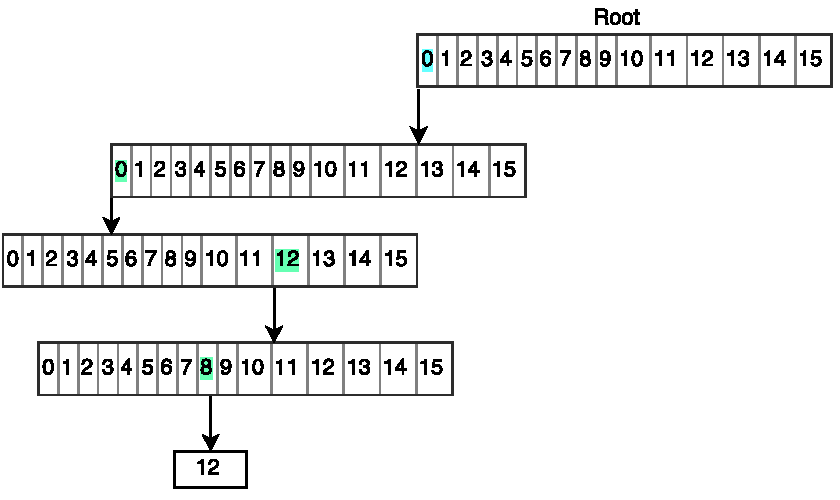
\includegraphics[scale=0.6]{tree}
\caption{ Traverse the tree for finding value according to key 200}
\centering

\end{figure}
\end{itemize}

Based on the characteristics that were explained, the structure of a node in the basic prefix tree has only 16 pointers. So for inserting a key/value pair into the tree, prefixes of the key will be calculated and based on the prefixes, we will traverse in the tree. If a node does not exist, we will create the node. Values are connected to the leaf nodes. So if We have inserted the same keys with two different values, values are connected to the leaf via linked list.  
 
 
\section{ Prefix tree with parity bits}
 
After building the tree, the main concept that should be taken care of in this thesis is to find the bit flips in the structure.
 
In the first solution, parity bits is used. As we have already explained, structure of the nodes contains of only pointers, so pointers in the nodes should be protected against bit flips otherwise a wrong value can be retrieved or we will access some parts of memory which are not in the range of our tree structure. For this purpose, parity bit has been calculated for each pointer in the node and 3 more bits is dedicated for redundancy of the parity bit because there is a chance that parity bit becomes corrupted itself.

 While inserting keys into the tree, parity bit is calculated for the child's pointer corresponding to the prefix of the key in the node and is set at the end of the node in the right place. After that three more redundant bits of the parity bit is also set. When a key is requested from the tree, during the traverse to reach the target node, parity bit for each of the pointers in this path is calculated and if 3 of the 4 parity bits which had been assigned for the pointer, matches the calculated parity bit, we assume that no bit flip has happened in the pointer otherwise a bit flip is reported.

For creating bit flips in the tree, we have created bit flips in a certain number of nodes. The number of bit flips is 1 or 3 bit flips. In this case, all the corrupted nodes were detected by using parity bits.
Although we could detect all the bit flips by using parity bits but parity bits always cause higher memory consumption since some bytes of the node should be assigned for the parity bits. The other problem with parity bit is that in case of multiple bit flips happening in a pointer, parity bit is not a good detection mechanism because only odd number of bit flips can be detected by it.  

\section{Keeping the nodes in a consecutive order in a pre allocated area of memory}

 Because of the mentioned reasons, the second solution is introduced which does not need redundant information on the nodes. Based on this solution, bit flips are detected by using the layout of the prefix tree. We keep the nodes in a continuous way inside the memory, so in case bit flip happens in the pointers which point to other nodes, it can be detected by knowing the exact address of the following node which can be extracted from the layout.(Node size is fixed) One problem in this approach is that structure of the tree depends on the inserted keys into it. Based on a set of keys, we might have a tree which is very disperse and based on another set of keys, tree can be dense. While preallocating memory for the tree, we have to save memory for a full tree, so that we can predict place of nodes in the memory. If a tree is disperse, using this structure is a waste of memory since we have to allocate a lot of memory while we might not use it. Only if we have a dense tree, this approach is beneficial. So we will assume that we are going to have a dense tree and we will pre allocate the memory for a full tree.

Based on the initial explanation on this method, the implementation has 4 steps:

\begin{enumerate}
  \item Finding out the density of the tree or insertion of which keys results in a dense tree.
  \item Pre allocating memory for a full tree and creation of the tree.
  \item Insertion of bit flips in the nodes.
  \item Evaluation of this method towards finding the bit flips.
\end{enumerate}  

\subsection{Finding density of the tree}

Density of the tree is not a fixed value and it changes based on the inserted keys. A set of keys can produce a completely dense tree, while another set can produce a disperse tree.
 We build the tree based on different set of keys. Different set of distributions of keys have been used for this purpose. The number of pointers in each node which are not null is called \textit{node degree}. \textit{Node degree} has been counted and if the average of this value among all the nodes is more than a defined value, we assume that the tree is dense enough. The distributions that are used for this purpose is as follows:
 \begin{itemize}
 \item Simple distribution (in which, keys are multiples of three)
 \item unifrom int distribution
 \item Poisson distribution
 \end{itemize}
Details of the implementation and the key distributions which are used are explained in the next chapter. As the result, using the simple distribution leads to a dense tree after insertion of around 2100 keys.
 
\subsection{Creation of the tree}
  
Until now we have chosen a set of keys to insert into the tree to have a dense tree. Based on this knowledge, we allocate memory for a full tree and start inserting keys into the tree and creating nodes. Since we have a large number of nodes, we can make the nodes into groups also. We will have four groups of nodes which each group is equivalent to each level in the tree. So We will keep the address of the start of the nodes in root level, first, second and third level in four variables. After each insertion into the tree, created nodes will be put in the places of memory which is preallocated for them. If we need to insert four nodes for insertion of a key, then the address of the second node should be calculated and put in the correct place in the first node and the address of the third node should be put in the correct place in the second node and finally the address of the fourth node should be put in the right place in node three. For getting a key from the tree, we can easily traverse to the correct node. The details of the implementation can be found in the next chapter. 

\subsection{Insertion of bit flips}

After creation of the tree, we will insert some bit flips in a number of nodes. After this insertion, we try to retrieve the keys. Since we know the exact address of the nodes, so whenever we want to get a key, we can go through the nodes by checking the address which is stored in the $i^{\text{th}}$ place of the node. We can calculate where the next node should be and compare it with what is written in the previous node. If these two values are the same, then we will keep traversing to the next node, otherwise a bit flip has been detected. Insertion of bit flips is done on one or three of the bits of some pointers in the third level. Insertion of bit flips is done by doing XOR bit wise on the pointer with a value that has one or three 1 bits in it and the rest of the bits are 0. In this case, just the bits which are XORed with 1 are flipped.  

\subsection{Evaluation}  

Based on this methodology, all the bit flips were detected but as we said before, this method needs pre allocation of memory for a full tree and in case we insert keys into the tree which sets only one pointer in a node, then we have allocated a full memory page when it was not necessary. Also If when we have large keys, then we might overflow the space in RAM. So in the next approach, we will see that we can avoid allocating space for a complete node when it is unnecessary.
 
\section{Using a new method for bit flip detection }

Another approach is shown for dealing with the problem of allocating a full set of nodes for insertion of a key. As a brief explanation, we have reserved memory for a full tree and some additional data in the virtual memory using \textit{mmap}, but allocation of a node in physical memory will happen only if there are more than one pointer descending from that node, otherwise, a key-value pair will be stored in physical memory instead of a bunch of nodes. In this approach, by using mmap, we can reserve virtual memory. When reserving memory via mmap, we are not allocating any memory from physical memory, but when we set a value to a part of the reserved memory, then operating system has to allocate the size of the memory page in physical memory. In this method, some ideas are taken from \textit{generalized trie} \cite{Boehm}. Based on the ideas which are taken from generalized trie, allocating a complete node, whenever we insert a key into the tree is highly memory consuming. In case there is only one child descending from a node, we do not need to create a whole node as child of that node. Instead, we can point to a key,value pair. If we have 32 bit keys and 32 bit values, each of these key,value pairs need 8 bytes of the memory while a whole node can take 16*8 bytes. The other clue which is taken from \textit{generalized trie} is that pointers which are stored in each node can be 32 bit pointers instead of 64 bits because we can just store the offset other than the whole address. With this optimization, node size will decrease to half. In order to locate the descending nodes, we can add the offset with the address of the level. 

 The other important point in this method is reserving memory for the tree structure. We reserved memory level by level and keep the starting address of each level in variables. 

At the moment we assume that we have 32 bit keys with prefix size 4. Then we will have 8 levels. We allocate memory for all the nodes in a level and also for all the key,value pairs.The number of key,value pairs is the same as the number of all the nodes in a level. For each node in the tree, we need one bit to show whether the node is set in the physical memory or not. If the bit is 1 then we assume that the node is set in the physical memory, otherwise a key-value pair is set instead of the node. Based on this knowledge, structure of tree in each level is as follows:
 
\begin{itemize}
\item Root level has one node with 16 pointers. Each pointer is 32 bits.   
 \item First level has 16 nodes. At the end of the level, we have 2 bytes which flag bits are kept in it.( one bit for each node). After that, we have $16*8$ bytes. Each of these 8 bytes is for storing one key-value pair. 
 \item Second level has 256 nodes. At the end of the level, we have 32 bytes to store the flag bits and $256*8$ bytes for storing the key-value pairs. 
 \item Third, fourth, fifth and sixth level will have $256*16$, $256*256$, $256*256*16$ and $256*256*256$ nodes accordingly. At the end of each of these levels, we will have enough bytes to store the flag bytes and key-value pairs.
 \item Seventh level will take up a lot of memory, so it has been divided into sub levels. We will have 8 sub levels. Each sub level will have $256*256*256*2$ nodes. At the end of each sub level, flag bytes are stored which take $256*256*64$ bytes. Starting address of each of these sub levels are kept in variables. At the end of these sub levels, key-value pairs for all the nodes in these levels are stored. Since we have $256*256*256*16$ nodes in the seventh level, we need $256*256*256*16*8$ bytes to store these pairs. Starting address to this part is also kept in a variable.
\end{itemize}

\begin{figure}[h]

\includegraphics[scale=0.09]{treestructure3}
\caption{ Tree structure in a memory optimized version}
\centering

\end{figure}

\subsection{Insertion in the tree}
 The first step for insertion of a key into the tree is to check if the key is the only key which is descended from the node(this can be done by checking the value stored in the corresponding bucket, if it is 0, then this key is the first key), then we can set the pointer in this bucket in a way that it points to a place of memory which holds a key,value pair. We know that key-value pair are stored at the end of each level and after the flag bytes. So for finding the correct address to put the key-value pair, we have to add the number of bytes which is reserved for storing all the nodes in the level and the number of flag bytes and also the correct offset for storing the key-value pair. We will put this address in the bucket. Having zero in the bucket can also mean that this bucket is pointing to the first node in the next level. So we have to distinguish between these two conditions. We can do this by checking the flag bit of the first node. If flag bit is set to zero, then we are sure that node is not set, so zero in the bucket meant null, otherwise if the flag bit is one, then we realize that node is set.
 
 If  bucket does not have a null value, then we have two conditions.\\
If we are checking the value in a bucket in the root, we should see if this value is more than $starting address of firstlevel+16*16*8$. (We have 16 nodes in first level. Each of the nodes have 16 buckets and size of each bucket is 8 bytes), in this case, we know that the pointer in that bucket, is already pointing to a key,value pair. So with inserting the new key, we should create a new node and insert the key which was stored in the key,value pair in the tree and also set the value in the bucket to the address of newly created node. We should free the memory which was allocated for the key-value pair. If the value in the bucket is less than $starting address of firstlevel+16*16*8$, then We conclude that a node has already been created, so there must have been multiple children from that bucket in the root. Then we should traverse to the next level in the tree and do the same check for the next node in the traverse and insert the value in the right place in the tree.

When we reach the sixth level in the tree, checks will be a bit different. In the seventh level, we have 8 sub levels as it was explained before. Based on \textit{key1} (which is the value of the least 4 bits of the key), we can recognize to look for the value in which sub level. As we said before, flag bytes of each sub level are stored at the end of the sub level. So we should check the flag bit of the corresponding node. If it is one, then we can continue our traverse in the tree and jump to the seventh level. Otherwise, we can look for the key-value pair at the end of the seventh level. We have already kept the starting address of the area which points to key-value pairs in seventh level. So with some calculations, we can get the correct key-value pair.          

\subsection{get a value from the tree considering the occurrence of bit flips }

We have considered that bit flips can happen in the pointers and flag bytes in each level. While searching for a key inside the tree, we will check the pointer value in the bucket of a node. We can locate the corresponding node in the next level based on values of \textit{key1},\textit{key2},\textit{key3},\textit{key4},\textit{key5},\textit{key6},\textit{key7} and \textit{key8}. First of all, we should find the corresponding flag bit for the node. Now we have two conditions:

\begin{itemize}

\item If flag bit is zero, then we should check the value stored in the bucket with the expected place of storing the key-value pair. If these two are the same, then we should check the key which is stored in the key-value pair with the actual key. If these two are also the same, then we can retrieve the value. We can do another check here. We have the flag bit set to zero, but a bit flip can have possibly happened in the bit. So we check the value stored in the bucket with the address of the node. In case of equality of these two values, we conclude that flag bit was actually corrupted. Otherwise a bit flip has happened in the key. 

\item If flag bit is set to one, then we should check the value stored in the bucket with the address of the corresponding node in the next level. If these two values are the same, then we can traverse to the next level in the tree to find the value. Otherwise, we can assume that a bit flip has happened in the flag bit and it is actually zero and not one. So we should check the value in the bucket with the expected address to store the key-value pair. If these two values are the same, then we should check the key which is stored in the key-value pair with the actual key, if these two are also the same, then we can retrieve the value and assume that a bit flip has happened in the flag bit.  
\end{itemize}

Based on the conditions which were discussed, this solution is bit flip resilient towards the bit flips which happens in the pointers and the flag bytes and also the key-value pairs.


\subsection{Insertion of bit flips in the tree}

Bit flips have been inserted in different levels in the tree. 

\chapter{Implementation}

Based on the methodologies that has been given in the last chapter, the implementation of them has been explained in details in this chapter.

\section{Implementation of the basic Prefix tree}

In order to start the implementation part, the first step is to make the initial structure of the prefix tree. It has been assumed that all the keys which are inserted into the tree are 16 bit keys. Prefix length is 4. So at the start, for doing insert operation or get operation, we would like to get the value of the prefixes. For this reason, in four iterations, we get the value of the least 4 bits of the key by doing \textit{and} operation between the key and $000F$. In the next iteration, we have to do right shift on the key for four bits and do the \textit{and} operation again. So in each iteration, after getting the prefix value, we keep it in \textit{key} variable. \textit{Key}'s value must be between 0 to 15. In the insert operation and in the first iteration, we have to check the pointer value which is set in the key's pointer of the root. If this value is null, Then we have to create a new node and set the address of the created node in key's pointer of the root. So the current node is the newly created node. In the next iteration, we will check the key's pointer in the current node and if it is null, we have to do the same action and create a node and set the key's pointer of the current node as the address of the newly created node. If key's pointer is not null, then we will just set the current node as the child node and jump to the next iteration. This process will go on for four iteration. In the last iteration, we have to set the pointer to the start of a linked list if the pointer is null. If pointer is not null, it means that a linked list is already created for this pointer and we can just add the value to the end of this linked list.     

When we want to get a value from the tree, we have to do the same iterations, but in case, one of the iterations leads to a null pointer, then we assume that key,value pair does not exist. 

\section{Implementation of the Prefix tree with parity bits}

As it is said before, in any index structure, bit flip can happen. In prefix tree, since each node contains only pointers, we should care about bit flips that happens in the pointers. For this purpose, we define the second type of implementation of prefix tree which contains parity bits inside the nodes. Here, we calculate parity bit for each pointer and keep 3 bits redundancy for that parity bit, in case the parity bit becomes corrupted itself. So by keeping 4 bits redundant data for each pointer, we will have $16*4 bits=8 byte$ redundant data for each node. So assuming that the implementation is done in a 64 bit system, we will need 136 byte memory for each node:


$8byte*16+8byte=136 byte$    

In the implementation of prefix tree with parity bits, parity bit will be calculated  while inserting a node into the tree. Referring to the same example in figure 3.1, while inserting key/value pair (200,12), at the start, a node will be created as a child of root which will be pointed to by pointer 0 in the root. So in 0th place in the root, address of the child node will be inserted. Parity bit for this address will be calculated and be put in the correct place in the root. Then we traverse to the created node, and the same action will be done. We will continue to the second and third node which is created in the tree and do the same thing. While reaching the leaf node, the value according to the key 200, will be pointed to by the pointer at 8th place in the leaf and the insertion is over.

The parity bits will be checked while trying to get a key/value pair from the tree. If we want to get the pair(200,12) which is already inserted into the tree, we will start the traverse from the root and check the pointer which is located in the 0th place of the root node. A calculation will be done in order to get the parity bit of the pointer. If the result of the parity is 1 and 3 of the 4 bits that are assigned for the parity data of this pointer are also 1, then we assume that the pointer is not corrupted, otherwise an error will be printed. This check will be done on the nodes which leads us to the corresponding leaf. If all the parity checks passes, then we will retrieve the value according to the key.

For testing this methodology, three steps are done:
\begin{itemize}
\item 20000 keys were added to the tree. 
\item A corruption is done on 1111 keys from the 20000 added keys by using setKey() function. Based on this function, one bit flip and another time 3 bit flips was done on the pointer.  
\item By using function getNode(), we tried to retrieve the key/value pairs of the 20000 inserted keys and all the corrupted keys have been detected but only if the number of bit flips in the addresses were one or three bits. If we have even number of bit flips, detection can not happen.  
\end{itemize}


\section{Implementation of the Prefix tree with having the nodes in a consecutive order in the memory}   

In the last method, it is obvious that using parity bits always causes extra memory consumption. In the new methodology which is given in this master thesis, we try to find out any corruption in the pointers by knowing the exact place of the nodes rather than using redundant data. 

\subsection{Finding the density of the tree}

For finding the density of the tree, two solutions has been suggested. In the first solution, the density of the tree is calculated based on the average number of children of the nodes in the tree. For this purpose, degree of a node( which defines the number of children of a node), is increased when another node is created and its address is assigned to one of the node's pointers. For keeping this data, map data structure in C++ has been used. So address of a node defines key and degree of the node defines value in a key/value pair in map, so whenever a pointer of a node is set to an address, the degree of that node will be increased in map data structure. After building the tree, all the pairs of the map data structure will be read and the average degree of the nodes will be calculated. If the result of the following equation is more than $0.625$, we assume that the tree is dense. 
\begin{equation}
Density = \frac{degree(n_1)+degree(n_2)+...+degree(n_N)}{N}
\end{equation}   

A set of keys have been inserted into the tree and density of the tree has been calculated. At the start, we inserted keys which were multiples of three. The second set of keys were produced by using \textit{Uniform int distribution}. The third set of keys were produced by using \textit{Poisson distribution}.

A set of results has been produced based on this test which is shown in the following figures.


\begin{figure}
  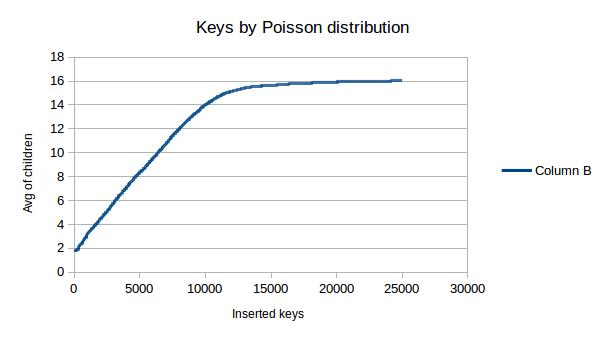
\includegraphics[scale=0.4]{Poissonchild}
  \caption{Average Number of children}
\end{figure}
  
\begin{figure}
  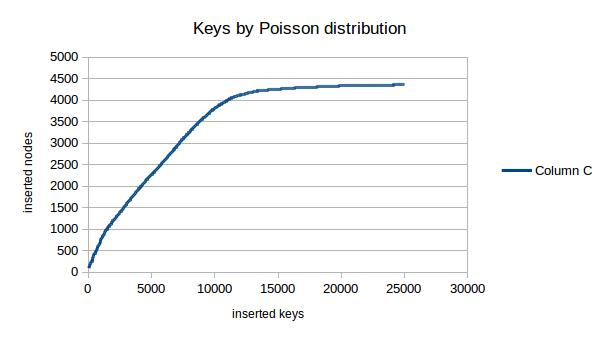
\includegraphics[scale=0.4]{Poissonnode}
  \caption{Number of inserted nodes}
\end{figure}

\begin{figure}
  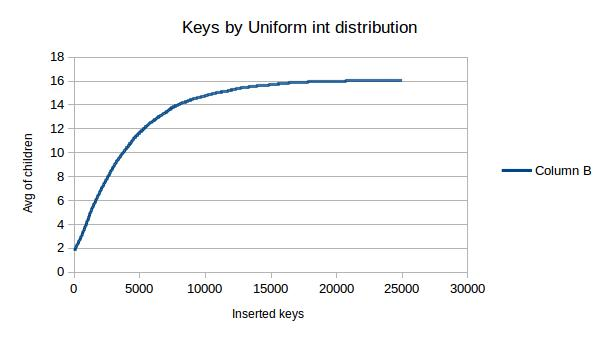
\includegraphics[scale=0.4]{uniformchild}
  \caption{Average Number of children}
\end{figure}

\begin{figure}
  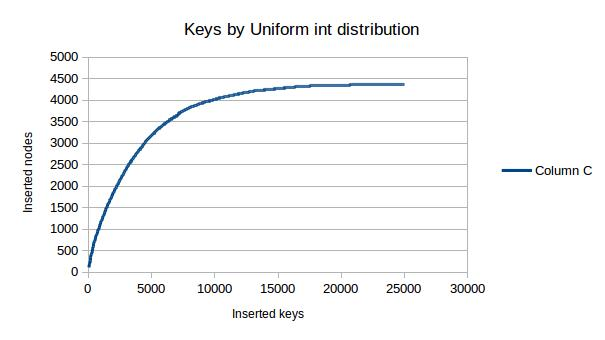
\includegraphics[scale=0.4]{uniformnode}
  \caption{Number of inserted nodes}
\end{figure}

\begin{figure}
 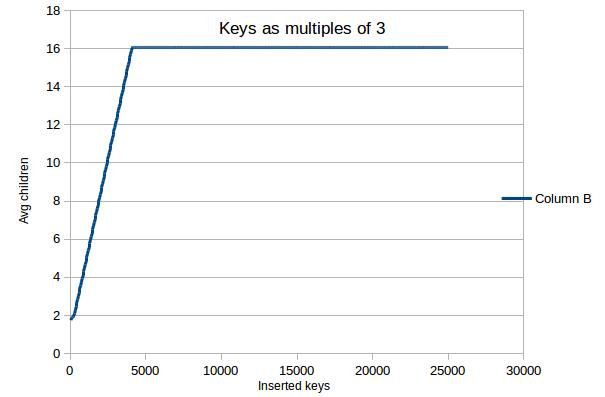
\includegraphics[scale=0.4]{mul3child}
 \caption{Average Number of children}
\end{figure}

\begin{figure}
 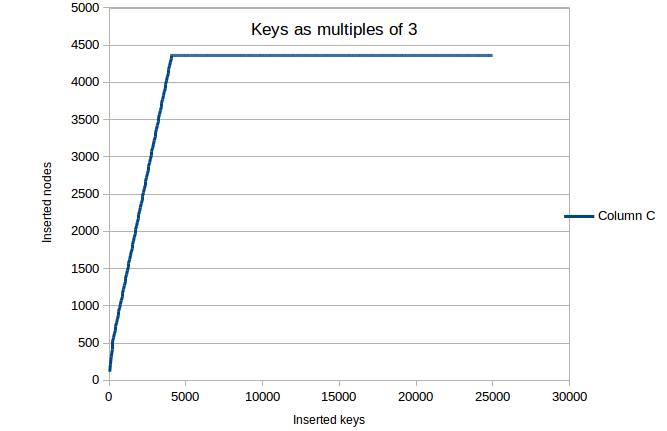
\includegraphics[scale=0.4]{mul3node}
 \caption{Number of inserted nodes}
\end{figure}


\begin{comment}
\begin{figure}
\centering
\begin{minipage}{.5\textwidth}
  \centering
  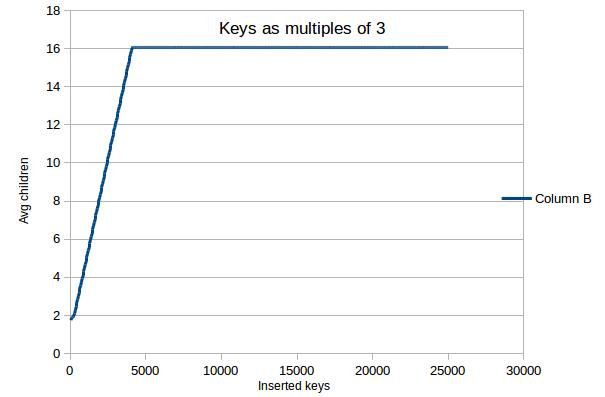
\includegraphics[scale=0.3]{mul3child}
  \caption{Average Number of children}
\end{minipage}%
\begin{minipage}{.5\textwidth}
  \centering
  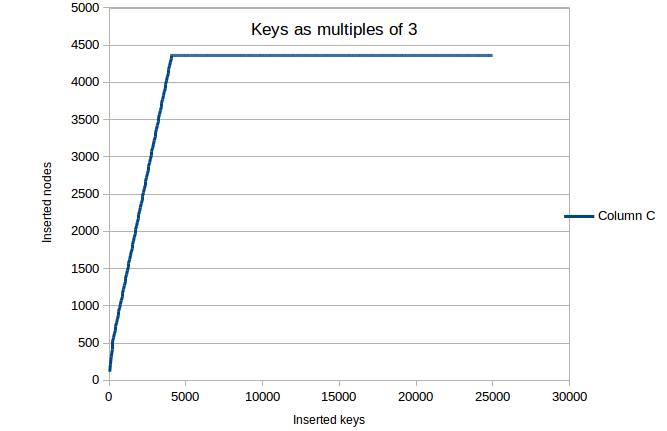
\includegraphics[scale=0.3]{mul3node}
  \caption{Number of inserted nodes}
\end{minipage}
\end{figure}
\end{comment}

Based on the charts in figure 4.2 and 4.3, we see the number of added nodes to the tree and the average number of children from each node while inserting keys into the tree. 50 to 25000 keys are added into the tree. As it is shown, more than 20000 nodes should be added to the tree till we reach a full tree. 

In figure 4.4 and 4.5, we can see the result for insertion of keys into the tree based on uniform int distribution. As it is shown, around 20000 keys need to be inserted into the tree in order to have a full tree. 

In figure 4.6 and 4.7, we can see the result for insertion of keys which are multiples of 3. As it is shown, around 4000 nodes need to be inserted into the tree in order to have a full tree which is a very big difference to using two other distributions. This huge difference is caused by the nature of uniform int distribution and Poisson distribution. Target of these distributions is to provide the random values. It is more likely that more keys need to be added in order to have more nodes in the tree and accordingly a denser tree in uniform int distribution and Poisson distribution than the method which provides the keys as multiples of three. There is no randomness in creating the keys which are multiples of three. Based on this result, keys which are multiples of three are for creating the tree.  




%In the second solution, we would like to find out that which part of the built tree is more dense. So based on this information we can find out with which set of keys, a dense tree will be produced. For this purpose, while insertion of every 20 keys into the tree, we keep the range of memory and the number of nodes which are added in this range. Then we can figure out approximately that how many nodes are added in each range and find the dense part of the memory. The next step is to build the tree with the keys that are added in that range.
\subsection{Creation of a dense tree with the new layout method}

Based on this method, allocation of memory is done for a full tree. So we allocate $16*8$ bytes for the root and keep the start address of the tree in a variable. After that we allocate $16*16*8$ bytes for the first level in the tree and keep the starting address of this level in a variable. After that we will keep every 16 nodes in one page and keep the address of the next page at the of previous page. So overall, we have kept starting address of the root, first level,second level and third level in 4 variables. Whenever we want to insert or access a key in the tree, we have to calculate address of the corresponding nodes based on one of those 4 addresses. The code for this implementation is in appendix B.

\subsection{Insertion of bit flips in the nodes}

As we said, we built the tree with the keys which are multiples of three. 20000 keys have been inserted and we chose the keys by reduction of multiples of 54 from 60000 for bit flip insertion. If we assume that third level is the leaf level, then we insert the bit flips in the second level of these keys.Inserting bit flips in an address is done by using $XOR$ function, So for insertion of one bit flip, we have to $XOR$ the address with a number which has one bit of binary set to one. While inserting bit flips in the second level of these keys, we keep the exact address that is corrupted in an array called \textit{corrupted}. If we have to insert bit flips in the same address again(if multiple keys share the same prefixes), then we will not keep this repetitive addresses in the array. When we try to get these 20000 keys, we know exactly to which addresses we should traverse, because all the nodes in the tree are located in order. So when we reach a node which contains the pointer which does not match with the layout, we check its address with the addresses which are kept in the \textit{corrupted} array. If it matches one of the addresses in the array, we increase the counter  \textit{countcorrupt}. At the end of getting all the keys from the tree, we compare the \textit{countcorrupt} with the actual number of corruptions in \textit{corrupted} array. As a result, all of the corruptions have been detected. The difference between this approach and parity approach is that by using parity bits, only an odd number of bit flips can be detected but by using this new structure, any number of bit flips can be detected.

\subsection{Evaluation}
The problem which comes in this solution is that, it is not a feasible solution when we have larger keys. So at the moment, we have pre allocated all the memory that we need for building a full tree. But when the size of the indexes increases, number of nodes will increase and will cause to a large memory consumption. If we still want to use this approach to keep the nodes in an order in memory based on breadth-first traverse and would not want to pre allocate all the memory which is needed, then we have to allocate memory whenever a node is created.

\section{Memory optimized version of prefix tree}

As it was discussed in the concept chapter, in this methodology, we will reserve virtual memory for a full tree( when we have 32 bit keys) plus all the space which is needed for key-value pairs and flag bytes. This is a lot of memory, but as we know, all of it is reserved in virtual memory and it will not cause any allocation in physical memory until we write a value in it.

In the following figure, a part of code which allocates memory for root, first and second level is shown.
  
\begin{figure}[h]
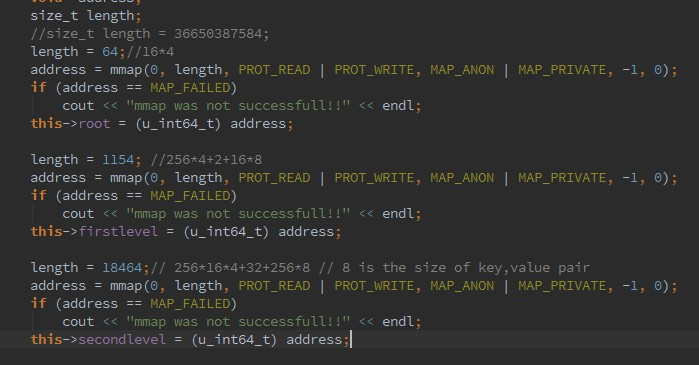
\includegraphics[scale=0.5]{memoryallocation}
\caption{Virtual memory allocation for the first, second and third level }
\centering
\end{figure}

By using \textit{mmap}, we can define to start the mapping from which address and also define the length of mapping. We have set PROT\_READ and PROT\_WRITE as the third argument, because pages can be read or written. As the fourth argument, MAP\_ANON and MAP\_PRIVATE has been set which defines that mapping is not backed by any file and its contents are initialized to zero. \cite{mmap}    

After allocating enough memory for the whole structure, we started inserting key-value pairs into the tree. Both key and value is assumed to be 32 bit. So they can have value of 4000000000 at most. At the worst case, we might need to traverse to the last level in the tree. So we have a for loop with 8 iterations. The only exception in these iterations is when we are in the sixth and seventh level. In the sixth level, we have to set the pointers to the nodes or key-value pairs in the seventh level. But as we said before, seventh level has 8 sub levels. So we need to figure out the sub level in which the node is. Also if we are in the last level, then values will sit in the place of pointers.( Pointers and values are both 32 bits)

There are four variables in the implementation named as \textit{ext}, \textit{extr2}, \textit{extr3} and \textit{extr4}. These variables will be updated in each iteration and would help us in finding the location of node in the next level, corresponding place for storing key-value pair if it is needed, place of the flag byte and the number of bytes which is needed for storing the flag bytes in each level. At the start of insertion:

\begin{itemize}
\item $extr=key1*4$ which shows the location of bucket in the root. (Each bucket has the size of 4 bytes)
\item $extr2=key1*8$ which shows the location of key-value pair at the end of first level. (Each key-value pair has the size of 8 bytes) 
\item $extr3=key1$ which shows that flag bit of the corresponding node should be in which flag byte at the end of the level.
\item $extr4=2$ Since we have 16 nodes in first level and we need one flag bit per node, so we need 2 bytes for storing the flag bits in the first level.
\end{itemize} 

In the second iteration, these values will change as follows:

\begin{itemize}
\item $extr=key1*4:16+key2*4$ which shows the location of bucket in the first level. 
\item $extr2=key1*8*16+key2*8$ which shows the location of key-value pair at the end of second level. 
\item $extr3=key1*16+key2$
\item $extr4=32$ Since we have 256 nodes in second level, so we need 32 bytes for storing the flag bits in the this level.
\end{itemize}

When we want to insert a key into the tree, the first thing to do is to find out if the flag bit of the corresponding node in the next level is set to one or zero. Based on the variables which were mentioned, we can locate the node and also the place of flag bit. If flag bit is set to one, then we can continue the iteration to the next level, otherwise, we have access to the key-value pair which is already inserted in the key-value pair area of that level. We should delete the key-value pair from that area and set the flag bit of the node to one and insert the key that was in the key-value area to the tree.

For getting a key from the tree, the first thing to do is to check the pointer which is stored in the bucket of the node. If pointer is less than a variable called \textit{cons}, then we realize that this bucket is pointing to a node rather than a key-value pair, so we should continue the iteration to find the corresponding value. Otherwise, bucket is pointing to a key-value pair and we can retrieve the value. \textit{Cons} actually holds an offset. For the first level, \textit{cons} is 1024 (16*16*4). From address 0 in the first level to address 1024, all the nodes are stored and flag bytes and key-value pairs are stored after this address (assuming that we are dealing with the offset address). In the second level, \textit{cons} will increase to 1024*16.

      

\begin{thebibliography}{1}

\bibitem{kolditz} M.Boehm,B.Schlegel,P.B Volk,U.Fischer,D.Habich {\em Online Bit Flip Detection for In-Memory B-Trees on Ureliable Hardware} 2014,TU Dresden 

\bibitem{Boehm}  {\em Efficient In-Memory Indexing with Generalized Prefix Trees} 2011,Tu Dresden

\bibitem{leca} T J.Lehman,M J.Carey {\em A study of Index Structures for Main Memory Database Management Systems} 1986: University of Wisconsin

\bibitem{Graefe} G.Graefe,R.Stonecipher {\em Efficient verification of B-tree integrity} : Hewlett-Packard laboratories,Microsoft.

\bibitem{harderror}
Hard error definition, \url{http://www.webopedia.com/TERM/H/hard_error.html}

\bibitem{softerror}
Hard error definition, \url{http://www.webopedia.com/TERM/H/soft_error.html}

\bibitem{reinhardt}
Reinhardt, Steven K.; Mukherjee, Shubhendu S. "Transient fault detection via simultaneous multithreading".(2000) ACM SIGARCH Computer Architecture News 28 (2): 25–36

\bibitem{mukherjee} Mukherjee, Shubhendu S.; Kontz, Michael; Reinhardt, Steven K. "Detailed design and evaluation of redundant multithreading alternatives".(2002) ACM SIGARCH Computer Architecture News 30 (2): 99.

\bibitem{vijaykumar} Vijaykumar, T. N.; Pomeranz, Irith; Cheng, Karl . "Transient-fault recovery using simultaneous multithreading".(2002) ACM SIGARCH Computer Architecture News 30 (2): 87.

\bibitem{soft} Soft errors detection, \url{https://en.wikipedia.org/wiki/Soft_error#Detecting_soft_errors}

\bibitem{immune} Immunity aware programming, \url{https://en.wikipedia.org/wiki/Immunity-aware_programming}


\bibitem{ramparity}
Immunity aware programming,\url{https://en.wikipedia.org/wiki/RAM_parity}

\bibitem{eccmemory} ECC memory,\url{https://en.wikipedia.org/wiki/ECC_memory}

\bibitem{Kissinger} Thomas Kissinger, Benjamin Schlegel, Dirk Habich, Wolfgang Lehner. "KISS-Tree: Smart Latch-Free In-Memory Indexing on Modern Architectures".(2012) In: Proceedings of the Eighth International Workshop on Data Management on New Hardware, Scottsdale, AZ, USA.
 
\bibitem{mmap}
Mmap manual,\url{ http://man7.org/linux/man-pages/man2/mmap.2.html}

\bibitem{ctrie} Ctrie,\url{https://en.wikipedia.org/wiki/Ctrie}

\bibitem{hamt}
Hash Array Mapped Trie, \url{https://en.wikipedia.org/wiki/Hash_array_mapped_trie}

\bibitem{calfcht}
Aleksandar Prokopec, Phil Bagwell, Martin Odersky, "Cache-Aware Lock-Free Concurrent Hash Tries". (2011) École Polytechnique Fédérale de Lausanne, Lausanne, Switzerland.

\bibitem{ctenbs}
Aleksandar Prokopec, Nathan G. Bronson, Phil Bagwell, Martin Odersky, "Concurrent Tries with Efficient Non-Blocking Snapshots". (2012) In: New Orleans, Louisiana, USA.

\bibitem{burst}
Steffen Heinz, Justin Zobel, Hugh E. Williams, "Burst Tries: A Fast, Efficient Data Structure for String Keys". (2002) In: School of Computer Science and Information Technology, RMIT University.
GPO Box 2476V, Melbourne 3001, Australia

\bibitem{splay}
 D.D. Sleator and R.E. Tarjan. "Self-adjusting binary search trees".(1985) In: AT\&T Bell Laboratories, Murray Hill, NJ. 

\end{thebibliography}

\end{document}